\documentclass[border=4pt]{standalone}
\usepackage[T1]{fontenc}
\usepackage{lmodern}
\renewcommand{\familydefault}{\sfdefault}
\usepackage[edges]{forest}
\tikzset{
  p/.style={draw=gray!60,fill=gray!12,inner sep=2pt,minimum height=5mm,font=\footnotesize},
  r/.style={p,fill=gray!35},
  h/.style={p,fill=white,dashed},
}
\forestset{calls/.style={for tree={folder,grow'=0,edge={gray!55!black},l sep=6mm,s sep=1.6mm,folder indent=3mm,p}}}
\begin{document}
\begin{tabular}{@{}l@{\hspace{14mm}}l@{}}
\begin{forest}calls
[main (setup and option 1),r,baseline,font=\footnotesize\bfseries
  [Initialize,r]
  [DisplayMenu,r
    [ReadNumber]]
  [AddBooking,r
    [ReadName]
    [ValidateBookingID,r
      [ReadBookingID [ReadNumber,h]]
      [FindBookingByID,r]]
    [ValidateMovieCode,r [ReadNumber,h]]
    [CountReservedSeats [GetSeatAddress]]
    [ValidateSeat,r [ReadNumber,h] [GetSeatAddress,h]]
    [ValidateCategory [ReadNumber,h]]
    [CalculateTicketPrice,r]
    [FindFreeSlot]
    [GetSeatAddress,h]]
]
\end{forest}
&
\begin{forest}calls
[main (options 2 to 5),r,baseline,font=\footnotesize\bfseries
  [CancelBooking,r
    [ReadBookingID,h]
    [FindBookingByID,h]
    [GetSeatAddress,h]]
  [DisplayTicket,r
    [ReadBookingID,h]
    [FindBookingByID,h]
    [PrintMovieName]
    [PrintCategoryName]]
  [DisplaySeatMap,r
    [ValidateMovieCode,h]
    [GetSeatAddress,h]
    [CountReservedSeats,h]]
  [DisplayStatistics,r
    [CalculateStatistics,r]
    [PrintMovieName,h]
    [DisplayHistogram,r]]
]
\end{forest}
\\[4mm]
\multicolumn{2}{@{}l@{}}{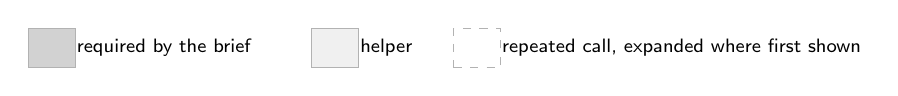
\begin{tikzpicture}[every node/.style={font=\scriptsize,anchor=west}]
\node[r,minimum width=6mm] at (0,0) {};\node at (0.5,0) {required by the brief};
\node[p,minimum width=6mm] at (3.6,0) {};\node at (4.1,0) {helper};
\node[h,minimum width=6mm] at (5.4,0) {};\node at (5.9,0) {repeated call, expanded where first shown};
\end{tikzpicture}}
\end{tabular}
\end{document}
